%% Antal Spector-Zabusky's UPenn thesis formatting skeleton, 2021
%%
%% Feel free to use any of this as necessary; you can contact me about it at
%% <antal.b.sz@gmail.com>.  This isn't all the styling in my thesis; it's mostly
%% limited to things that help you satisfy the formatting guidelines instead of
%% style choices.  It does not contain styling for things I didn't include, such
%% as a dedication or an index.  I wrote this for a CS thesis, so some details
%% may be specific to that.
%%
%% This should follow the formatting guidelines from
%% <https://guides.library.upenn.edu/dissertation_manual/formatting> as of
%% Spring 2021.
%%
%% Explanatory comments are annotated with ASZ; you can delete them if you
%% want.
%%
%% Good luck!

%% ASZ: 12 point font, single-sided (don't alternate left/right margins), and
%% sensible defaults.
\documentclass[12pt,oneside]{amsbook}

%%%%%%%%%%%%%%%%%%%%%%%%%%%%%%%%%%%%%%%%%%%%%%%%%%%%%%%%%%%%%%%%%%%%%%%%%%%%%%%%

%% ASZ: My usual "make things look nice and behave well" block
\usepackage[utf8]{inputenc}
\usepackage[T1]{fontenc}
\usepackage{lmodern}
\usepackage{microtype}
\usepackage{accsupp}
\usepackage{etoolbox}
\usepackage{newunicodechar}
\usepackage[dvipsnames,svgnames,x11names]{xcolor}
\usepackage{hyperref}
\usepackage{xspace}
\usepackage[
  backend=biber]{biblatex}
\addbibresource{bibliography.bib}

\usepackage{draft} % local
\newif\ifdraft\drafttrue
\newnote{lys}{BrickRed}
\newnote{bcp}{Chocolate}
\newnote{sz}{violet}

\def\sectionautorefname{Section}
\def\subsectionautorefname{Subsection}
\def\subsubsectionautorefname{Subsubsection}
\def\lstnumberautorefname{Line}
\usepackage{textcomp,listings,lstparams,lstcoq,graphicx}
\lstdefinestyle{customcoq}{
  language=Coq,
  literate={<>}{$\ne$}1
  {->}{$\to$}1
}
\lstdefinestyle{json}{
  language=Coq,
  literate={@}{$@$}1
  {this}{$\ottkw{this}$}4
  {ref}{$\ottkw{ref}$}3
}
\lstdefinestyle{customc}{
  language=C
}
\newcommand{\http}{HTTP/1.1\xspace}
\newcommand{\inlinec}[1]{\lstinline[style=customc]{#1}}
\newcommand{\ilc}[1]{\lstinline[style=customcoq]{#1}}
\newcommand{\ilj}[1]{\lstinline[style=json]{#1}}

%% ASZ: `amsbook` didn't style `\paragraph`s appropriately
\patchcmd{\paragraph}{\normalfont}{\itshape}
  {} % Success
  {\GenericError
     {} % Continuation for \MessageBreak (unused)
     {Could not redefine \string\paragraph\space to be italic}
     {(This is a hack in the preamble.)} % Where to look for more info?
     {I tried to replace \string\normalfont\space with \string\itshape, but I
      couldn't.}}

%% ASZ: Change the spacing in the list of figures – I don't know if you need
%% this or not
\makeatletter
\patchcmd{\l@figure}{1.5pc}{2.25pc}
  {} % Success
  {\GenericError
     {} % Continuation for \MessageBreak (unused)
     {Could not fix the spacing in the list of figures}
     {(This is a hack in the preamble.)} % Where to look for more info?
     {I tried to replace the 1.5pc figure number--figure description separation
      with a 2.25pc separation in \string\l@figure\space, but I couldn't.}}

%% ASZ: I like it when tables of contents know where they are
\patchcmd{\@starttoc}{\ifx\contentsname}{\iffalse}
  {} % Success
  {\GenericError
     {} % Continuation for \MessageBreak (unused)
     {Could not add a line to the table of contents for itself}
     {(This is a hack in the preamble.)} % Where to look for more info?
     {I tried to replace the check in \string\@starttoc\space that suppresses a
      table of contents entry for the table of contents, but I couldn't.}}

%% ASZ: The other half of the above
\patchcmd{\@starttoc}{\@tocwrite}{\phantomsection\@tocwrite}
  {} % Success
  {\GenericError
     {} % Continuation for \MessageBreak (unused)
     {Could not add link targets to the table of contents/front matter lists}
     {(This is a hack in the preamble.)} % Where to look for more info?
     {I tried to add \string\phantomsection\space to \string\@starttoc\space so
      that it would generate hyperlink targets, but I couldn't.}}
\makeatother

%% ASZ: Set the page layout correctly: 1.5" margins on the left, 1" margins
%% everywhere else, page numbers count
\usepackage{fullpage}
\usepackage[margin=1in,left=1.5in,includeheadfoot]{geometry}

%% ASZ: Make footnote numbers run continuously, rather than restart at the start
%% of every chapter; this is required by the formatting guidelines
\counterwithout*{footnote}{chapter}

%% ASZ: I found these to be much clearer
\numberwithin{section}{chapter}
\numberwithin{figure}{chapter}
\numberwithin{equation}{chapter}

%%%%%%%%%%%%%%%%%%%%%%%%%%%%%%%%%%%%%%%%%%%%%%%%%%%%%%%%%%%%%%%%%%%%%%%%%%%%%%%%

%% ASZ: This is a package for generating and styling the various "preliminary
%% pages": title page, copyright page, and abstract
\usepackage{upenn-dissertation-preliminary-pages} % local
\NoSignatureLines %% ASZ: For COVID – turns off adding lines on the title page
                  %% for people to sign.  The default is \YesSignatureLines.
\SingleSpaceAbstract %% ASZ: I think it looks better than a double-spaced
                     %% abstract, although in deference to the guidelines,
                     %% \DoubleSpaceAbstract is the default.

%% ASZ: Fill out your own information here :-)  Some notes:
%%
%% * You need to specify your advisor, the graduate chair, and your committee
%%   members, even if there's overlap between these groups.
%%
%%   * Your external committee member(s) need both their title and their
%%   affiliation; below, just imagine that everyone but Gödel works at Penn.
%%
%% * Note that some of the faculty involved for you may be assistant or
%%   associate professors (but I couldn't bring myself to apply that title to
%%   any of these luminaries).  I don't believe extra titles (e.g., "ENIAC
%%   President's Distinguished Professor") are necessary.
%%
%% * Only one committee chair is supported; you'll need to modify
%%   `upenn-dissertation-preliminary-pages.sty` (or email me about it) to change
%%   that.
%%
%% * When rendering the title page, your chair (if present) comes first,
%%   followed by the rest of the committee in the same order as in the TeX.
%%
%% * Using a Creative Commons license is optional, and thus so is specifying
%%   `\creativecommons`.  If you want to use one, choose from the licenses
%%   available at <https://creativecommons.org/licenses/>, perhaps by using the
%%   license chooser at <https://creativecommons.org/choose/>.  You'll have to
%%   copy the name of the  license (including the short string) and the URL
%%   separately, as you can see with the text below (the license I used); I
%%   didn't build a LaTeX Creative Commons license parser (yet? :-)).
\title{Language-Based Interactive Testing}
\author{Yishuai Li}
\graduategroup{Computer and Information Science}
\graduationyear{2022}
\advisor{Benjamin C. Pierce}{Professor of Computer and Information Science}
\graduatechair{Mayur Naik}{Professor of Computer and Information Science}
\committeechair{Steve Zdancewic}{Professor of Computer and Information Science}
\committeemember{Mayur Naik}{Professor of Computer and Information Science}
\committeemember{Boon Thau Loo}{Professor of Computer and Information Science}
\committeemember{John Hughes}{Professor of Computing Science, Chalmers University of Technology}
\creativecommons
  {Attribution-Share\-Alike 4.0 International (CC BY-SA 4.0)}
  {https://creativecommons.org/licenses/by-sa/4.0/}

\begin{document}

%% ASZ: Roman page numbers
\frontmatter

\maketitle

\copyrightpage

\chapter*{Acknowledgments}
\label{chap:acknowledgments}

Lorem ipsum dolor sit amet, consectetur adipiscing elit, sed do eiusmod tempor
incididunt ut labore et dolore magna aliqua. Ut enim ad minim veniam, quis
nostrud exercitation ullamco laboris nisi ut aliquip ex ea commodo
consequat. Duis aute irure dolor in reprehenderit in voluptate velit esse cillum
dolore eu fugiat nulla pariatur. Excepteur sint occaecat cupidatat non proident,
sunt in culpa qui officia deserunt mollit anim id est laborum.

%% ASZ: ... the rest of your acknowledgments go here ...

%% ASZ: The `upenn-dissertation-preliminary-pages` package will correctly style
%% this, including your thesis name, your name, and your advisor's name.
\begin{abstract}{chap:abstract}
  Lorem ipsum dolor sit amet, consectetur adipiscing elit, sed do eiusmod tempor
  incididunt ut labore et dolore magna aliqua. Ut enim ad minim veniam, quis
  nostrud exercitation ullamco laboris nisi ut aliquip ex ea commodo
  consequat. Duis aute irure dolor in reprehenderit in voluptate velit esse
  cillum dolore eu fugiat nulla pariatur. Excepteur sint occaecat cupidatat non
  proident, sunt in culpa qui officia deserunt mollit anim id est laborum.
\end{abstract}

\tableofcontents
\listoffigures

%% ASZ: Arabic page numbers
\mainmatter

\chapter{Introduction}
\label{chap:introduction}

The security and robustness of networked systems rest in large part on the
correct behavior of various sorts of servers.  This can be validated either by
full-blown verification or model checking against formal specifications, or
less expensively by rigorous testing.

Rigorous testing requires a rigorous specification of the protocol that we
expect the server to obey.  Protocol specifications can be written as (i) a {\em
  server model} that describes {\em how} valid servers should handle messages,
or (ii) a {\em property} that defines {\em what} server behaviors are valid.
From these specifications, we can conduct (i) {\em model-based
  testing}~\cite{broy2005model} or (ii) {\em property-based testing}~\cite{pbt},
respectively.

When testing server implementations against protocol specifications, one
critical challenge is {\em nondeterminism}, which arises in two forms---we call
them (1) {\em internal nondeterminism} and (2) {\em network nondeterminism}:

(1) {\em Within} the server, correct behavior may be \mbox{underspecified}.
For example, to handle HTTP conditional requests \cite{rfc7232}, a server
generates strings called entity tags (ETags), but the RFC specification does
not limit {what} values these ETags should be.  Thus, to create test
messages containing ETags, the tester must remember and reuse the ETags it
has been given in previous messages from the server.

(2) {\em Beyond} the server, messages and responses between the server and
different clients might be delayed and reordered by the network and
operating-system buffering.  If the tester cannot control how the execution
environment reorders messages---{\it e.g.,} when testing over the Internet---it
needs to specify what servers are valid as observed over the network.

These sources of nondeterminism pose challenges in various aspects of testing network
protocols: (i) The {\em validation logic} should accept various implementations,
as long as the behavior is included in the specification's space of
uncertainties; (ii) To capture bugs effectively, the {\em test harness} should
generate test cases based on runtime observations; (iii) When {\em shrinking} a
counterexample, the test harness should adjust the test cases based on the
server's behavior, which might vary from one execution to another.

To address these challenges, I introduce symbolic languages for writing
specifications and representing test cases:

(i) The specification is written as a reference implementation---a
nondeterministic program that exhibits all possible behavior allowed by
the protocol.  Inter-implementation and inter-execution uncertainties are
represented by symbolic variables, and the space of nondeterministic behavior is
defined by all possible assignments of the variables.

The validation logic is derived from the reference implementation, by {\em
  dualising} the server-side program into a client-side observer.

(ii) Test generation heuristics are defined as computations from the observed
trace (list of sent and received messages) to the next message to send.  I
introduce a symbolic intermediate representation for specifying the relation
between the next message and previous messages.

(iii) The symbolic language for generating test cases also enables effective
shrinking of test cases.  The test harness minimizes the counterexample by
shrinking its symbolic representation.  When running the test with a shrunk
input, the symbolic representations can be re-instantiated into request messages
that reflect the original heuristics.

\paragraph{Thesis claim}
Symbolic abstract representation can address challenges in testing networked systems with uncertain behavior.
Specifying protocols with symbolic reference implementation enables validating
the system's behavior systematically.  Representing test input as abstract
messages allows generating and shrinking interesting test cases.  Combining
these methods result in a rigorous tester that can capture protocol violations
effectively.

This thesis is structured as follows:

\chapter{Challenges}
\label{chap:challenges}
The Deep Specification project~\cite{deepspec} aims at building a web server and
guarantee its functional correctness with respect to formal specification of the
network protocol.

\http requests can be conditional: if the client has a local copy of some
resource and the copy on the server has not changed, then the server needn't
resend the resource.  To achieve this, an \http server may generate a short
string, called an ``entity tag'' (ETag), identifying the content of some
resource, and send it to the client:
\begin{lstlisting}[style=customc]
/* Client: */
GET /target HTTP/1.1

/* Server: */
HTTP/1.1 200 OK
ETag: "tag-foo"
... content of /target ...
\end{lstlisting}
The next time the client requests the same resource, it can include the ETag in
the GET request, informing the server not to send the content if its ETag still
matches:

\begin{lstlisting}[style=customc]
/* Client: */
GET /target HTTP/1.1
If-None-Match: "tag-foo"

/* Server: */
HTTP/1.1 304 Not Modified
\end{lstlisting}

If the tag does not match, the server responds with code 200 and the updated
content as usual.  Similarly, if a client wants to modify the server's resource
atomically by compare-and-swap, it can include the ETag in the PUT request as
\inlinec{If-Match} precondition, which instructs the server to only update the
content if its current ETag matches.

Thus, whether a server's response should be judged {\em valid} or not
depends on the ETag it generated
when creating the resource.  If the tester doesn't know the server's internal
state ({\it e.g.}, before receiving any 200 response including the ETag), and
cannot enumerate all of them (as ETags can be arbitrary strings), then it needs
to maintain a space of all possible values, narrowing the space upon further
interactions with the server.

\begin{figure}
  \begin{lstlisting}[style=customcoq,mathescape=true]
(* update : (K -> V) * K * V -> (K -> V) *)
let check (trace  : stream http_message,
           data   : key -> value,
           is     : key -> etag,
           is_not : key -> list etag) =
  match trace with
  | PUT(k,t,v) :: SUCCESSFUL :: tr' =>
    if t $\in$ is_not[k] then reject
    else if   is[k] == unknown
            $\vee$ strong_match(is[k],t)
         then let d' = update(data,k,v)     in
              let i' = update(is,k,unknown) in
              let n' = update(is_not,k,[])  in
       (* Now the tester knows that
        * the data in [k] is updated to [v],
        * but its new ETag is unknown. *)
              check(tr',d',i',n')
         else reject
  | PUT(k,t,v) :: PRECONDITION_FAILED :: tr' =>
    if strong_match(is[k],t) then reject
    else let n' = update(is_not, k, t::is_not[k])
      (* Now the tester knows that
       * the ETag of [k] is other than [t]. *)
         in check(tr',data,is,n')
  | GET(k,t) :: NOT_MODIFIED :: tr' =>
    if t $\in$ is_not[k] then reject
    else if is[k] == unknown $\vee$ weak_match(is[k],t)
         then let i' = update(is,k,t) in
       (* Now the tester knows that
        * the ETag of [k] is equal to [t]. *)
              check(tr',data,i',is_not)
         else reject
  | GET(k,t0) :: OK(t,v) :: tr' =>
    if weak_match(is[k],t0) then reject
    else if data[k] $\neq$ unknown $\wedge$ data[k] $\neq$ v
         then reject
         else let d' = update(data,k,v) in
              let i' = update(is,  k,t) in
       (* Now the tester knows
        * the data and ETag of [k]. *)
              check(tr',d',i',is_not)
  | _ :: _ :: _  => reject
  end
  \end{lstlisting}
  \caption{Ad hoc tester for \http conditional requests, demonstrating how
    tricky it is to write the logic by hand.  The checker determines whether a
    one-client-at-a-time \ilc{trace} is valid or not.  The trace is represented
    as a stream (infinite linked list, constructed by ``\ilc{::}'') of HTTP
    messages sent and received.
    \ilc{PUT(k,t,v)} represents a PUT
    request that changes \ilc{k}'s value into \ilc{v} only if its ETag matches
    \ilc{t}; \ilc{GET(k,t)} is a GET request for \ilc{k}'s value only if its
    ETag does not match \ilc{t}; \ilc{OK(t,v)} indicates the request target's
    value is \ilc{v} and its ETag is \ilc{t}.  The tester maintains three
    sorts of  knowledge about
    the server: \ilc{data} stored for each content, what some
    ETag \ilc{is} known to be equal to, and what some ETag \ilc{is_not} equal
    to.
  }
  \label{fig:etag-tester}
\end{figure}

It is possible, but tricky, to write an ad hoc tester for \http by manually
``dualizing'' the behaviors described by the informal specification documents
(RFCs).  The protocol document describes {\em how} a valid server should handle
requests, while the tester needs to determine {\em what} responses received from
the server are valid.  For example, ``If the server has revealed some resource's
ETag as \inlinec{"foo"}, then it must not reject requests targetting this
resource conditioned over \inlinec{If-Match: "foo"}, until the resource has been
modified''; and ``Had the server previously rejected an \inlinec{If-Match}
request, it must reject the same request until its target has been modified.''
\autoref{fig:etag-tester} shows a hand-written tester for checking this bit of
ETag functionality; we hope the reader will agree that this testing logic is not
straightforward to derive from the informal ``server's eye'' specifications.

Networked systems are naturally concurrent, as a server can be connected with
multiple clients.  The network might delay packets indefinitely, so messages
sent via different channels may be reordered during transmission.  When the
tester observes messages sent and received on the client side, it should allow
all observations that can be explained by the combination of a valid server + a
reasonable network environment between the server and clients.

\chapter{Prior Practices in Interactive Testing}
\label{chap:practices}
\section{Specification Languages}

\subsection{Property-based specification with QuickChick}
My first formal specification of \http was written as
QuickChick~\cite{quickchick} properties, which takes a trace of requests, and
determines whether the traces is valid per protocol specification, like that
shown in \autoref{fig:etag-tester}.  The specification implemented a constraint
solving logic by hand, making it hard to scale when the protocol becomes more
complex, as discussed in \autoref{sec:challenges}

\subsection{Model-based specification with ITrees}
To write specifications for protocols' rich semantics, I employed ``interaction
tree'' (ITree), a generic data structure for representing interactive programs,
introduced by \textcite{itree}.  ITree enables specifying protocols as monadic
programs that model valid implementations' possible behavior.  The model program
can be interpreted into a tester program, to be discussed in
\autoref{sec:spec-to-test}.

\begin{figure}
  \begin{lstlisting}[style=customcoq]
CoInductive itree (E : Type -> Type) (R : Type) :=
| Ret (r : R)
| Vis {X : Type} (e : E X) (k : X -> itree E R)
| Tau (t : itree E R).

Inductive event (E : Type -> Type) : Type :=
| Event : forall X, E X -> X -> event E.

Definition trace E := list (event E)

Inductive is_trace E R
  : itree E R -> trace E -> Prop := ...
  (* straightforward definition omitted *)
 \end{lstlisting}
  \caption{Interaction trees and their traces of events.}
  \label{fig:itrees}
\end{figure}

Figure~\ref{fig:itrees} defines the type \ilc{itree E R}.  The definition is
\textit{coinductive}, so that it can represent potentially infinite sequences of
interactions, as well as divergent behaviors.  The parameter \ilc{E} is a type
of \textit{external interactions}---it defines the interface by which a
computation interacts with its environment.  \ilc{R} is the \textit{result} of
the computation: if the computation halts, it returns a value of type \ilc{R}.

There are three ways to construct an ITree. The \ilc{Ret r} constructor
corresponds to the trivial computation that halts and yields the value
\ilc{r}. The \ilc{Tau t} constructor corresponds to a silent step of
computation, which does something internal that does not produce any visible
effect and then continues as \ilc{t}.  Representing silent steps explicitly with
\ilc{Tau} allows us, for example, to represent diverging computation without
violating Coq's guardedness condition~\cite{coinduction}:

\begin{lstlisting}[style=customcoq]
CoFixpoint spin {E R} : itree E R := Tau spin.
\end{lstlisting}

The final, and most interesting, way to build an ITree is with the \ilc{Vis X e
  k} constructor.  Here, \ilc{e : E X} is a ``visible'' external effect
(including any outputs provided by the computation to its environment) and
\ilc{X} is the type of data that the environment provides in response to the
event.  The constructor also specifies a continuation, \ilc{k}, which produces
the rest of the computation given the response from the environment.  \ilc{Vis}
creates branches in the interaction tree because \ilc{k} can behave differently
for distinct values of type \ilc{X}.

Here is a small example that defines a type \ilc{IO} of output or input
interactions, each of which works with natural numbers.  It is then
straightforward to define an ITree computation that loops forever, echoing each
input received to the output:

\begin{lstlisting}[style=customcoq]
Variant IO : Type -> Type :=
| Input  : IO nat
| Output : nat -> IO ().

CoInductive echo : itree IO () :=
  Vis Input (fun x => Vis (Output x) (fun _ => echo)).
\end{lstlisting}

\section{From Specification to Tester}
\label{sec:spec-to-test}
From an ITree specification, I conducted ``offline'' testing, which takes a
trace and determines its validity~\cite{cpp19}, and ``online'' testing, where
the specification is derived into a client program that validates the system
under test interactively~\cite{issta21}.

\subsection{Offline testing of swap server}
I started with testing a simple ``swap server''~\cite{cpp19}, specified in
\autoref{fig:linear-spec}.  The specification says that the server can either
accept a connection with a new client (\ilc{obs_connect}) or else receive a
message from a client over some established connection (\ilc{obs_msg_to_server}
\ilc{c}), send back the current stored message (\ilc{obs_msg_from_server}
\ilc{c} \ilc{last_msg}), and then start over with the last received message as
the current state.

\begin{figure}
\begin{lstlisting}[style=customcoq]
CoFixpoint linear_spec' (conns : list connection_id)
           (last_msg : bytes) : itree specE unit :=
  or ( (* Accept a new connection. *)
       c <- obs_connect;;
       linear_spec' (c :: conns) last_msg )
     ( (* Exchange a pair of messages on a connection. *)
       c <- choose conns;;
       msg <- obs_msg_to_server c;;
       obs_msg_from_server c last_msg;;
       linear_spec' conns msg ).

Definition linear_spec := linear_spec' [] zeros.
\end{lstlisting}
\caption{Linear specification of the swap server.  In the \ilc{linear_spec'}
  loop, the parameter \ilc{conns} maintains the list of open connections, while
  \ilc{last_msg} holds the message received from the last client (which will be
  sent back to the next client).  The server repeatedly chooses between
  accepting a new connection or doing a receive and then a send on some existing
  connection picked in the list \ilc{conns}.  The linear specification is
  initialized with an empty set of connections and a message filled with zeros.}
\label{fig:linear-spec}
\end{figure}

To test this swap server, I wrote a client program that interacts with the
server and produces a trace of requests and responses, and a function that
determines whether the trace $t$ is a trace of the linear specification $s$ {\it
  i.e.} whether \ilc{is_trace s t} in \autoref{fig:itrees} holds.

To network nondeterminism, the checker enumerates all possible server-side
message orders that can explain the client-side observations, and checks if any
of them satisifes the protocol specification.

\subsection{Online testing of HTTP}
To test protocols with internal nondeterminism ({\it e.g.} HTTP) effectively, I
introduced a symbolic representation for the server's invisible choices, as
shown in \autoref{fig:if-match-model}.  I then defined a TCP network model in
\autoref{fig:tcp-model}.  Combining the server and network models produces a
model program that exhibits all valid observations, considering both internal
and network nondeterminism.

\begin{figure}
\begin{lstlisting}[style=customcoq]
(* matches : (etag * exp etag) -> exp bool *)
(* IF      : (exp bool * T * T) -> T       *)
let put (k    : key,
         t    : etag,
         v    : value,
         data : key -> value,
         xtag : key -> exp etag) =
    IF (matches(t, xtag[k]),
    (* then *)
       xt := fresh_tag();
       let xtag' = update(xtag, k, xt) in
       let data' = update(data, k, v)  in
       return (OK, xtag', data'),
    (* else *)
       return (PreconditionFailed, xtag, data))
\end{lstlisting}
\caption{Symbolic model handling conditional PUT request.  The model maintains
  two states: \ilc{data} that maps keys to their values, and \ilc{xtag} that
  maps keys to symbolic variables that represent their corresponding ETags.
  Upon receiving a PUT request conditioned over ``If-Match: \ilc{t}'', the
  server should decide whether the request ETag \ilc{matches} that stored in the
  server.  Upon matching, the server processes the PUT request, and represents
  the updated value's ETag as a fresh variable.
}
\label{fig:if-match-model}
\end{figure}

\begin{figure}
\begin{lstlisting}[style=customcoq]
let tcp (buffer : list packet) =
    let absorb =
        pkt := recv();
        tcp (buffer ++ [pkt]) in
    let emit =
        let pkts = oldest_in_each_conn(buffer) in
        pkt := pick_one(pkts);
        send(pkt);
        tcp (remove(pkt, buffer)) in
    or (absorb, emit)
\end{lstlisting}
\caption{Network model for concurrent TCP connections.  The model maintains a
  \ilc{buffer} of all packets en route.  In each cycle, the model may
  nondeterministically branch to either absorb \ilc{or} emit a packet.  Any
  absorbed packet is appended to the end of buffer.  When emitting a packet, the
  model may choose a connection and send the oldest packet in it.  }
\label{fig:tcp-model}
\end{figure}

From the server and network models, I derived a tester client that interacts
with servers over the network, and validates the observations against the
protocol specification, as shown in \autoref{fig:framework}.

Using this automatially derived tester program, I have found violations against
HTTP/1.1 in the latest version of both Apache and Nginx.  More details are
explained in \textcite{issta21}.

\subsection{Key innovation}
To solve the problem of ``determinining whether an observation is explainable by
a nondeterministic program'', I reduced it into a constraint
satisfiability: Although the tester doesn't know the server and network's exact
choices, it can gain some knowledge of these invisible choices by observing the
trace of messages.  If the invisible choices are represented as symbolic
variables, then an observed trace is valid if there exists some value for the
variables that explains this trace, which can be determined by a constraint
solver.

\begin{figure}
  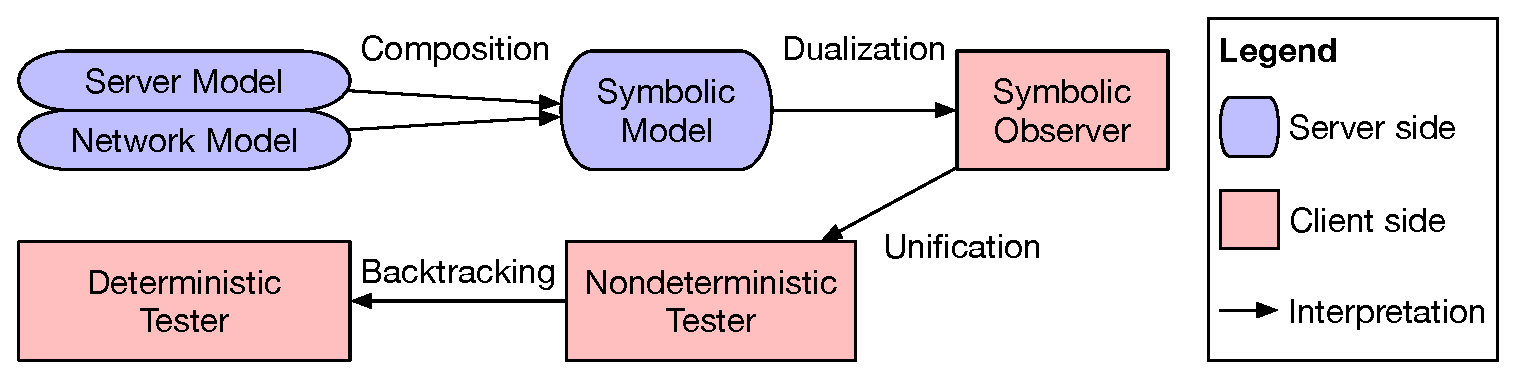
\includegraphics[width=\linewidth]{figures/framework}
  \caption{Deriving tester program from specification}
  \label{fig:framework}
\end{figure}

\chapter{Theories Developed for Interactive Testing}
\label{chap:theories}
During the testing practice in \autoref{chap:practices}, the tester's quality was
evaluated by mutation testing, {\it i.e.} running the tester against buggy
implementations to see if it rejects.  To formally prove that the tester is
good, I develop a theory for reasoning on testers' good properties.

{\em Interactive testing} is a process that reveals the SUT's interactions and
determines whether it satisfies the specification.  There are two kinds of
interactions: (1) {\em inputs} that the tester can specify, and (2) {\em
  outputs} that are observed from the SUT.  In particular, when testing
networked systems, the input is a message sent by the tester, and the output is
a message received from the SUT.

When viewing the SUT as a function from inputs to outputs, we can test the
system by (1) providing an input, (2) get the output, and (3) validating the
input-output pair.  This process is called {\em synchronous testing}.

However, the nature of networked systems is that multiple messages might arrive
at the system simultaneously, and a high-throughput system should handle the
messages concurrently.  To check the system's validity upon concurrent inputs,
the tester should send multiple messages, rather than executing ``one client at
a time''.  This non-blocking process is called {\em asynchronous testing}.

My goal is to formalise the techniques in \textcite{issta21} into a generic
theory for asynchronous testing.

A tester consists of two parts: (i) a test harness that interacts with the SUT
and observes the interactions, and (ii) a validator that determines whether the
observations satisfy the specification.

The test harness needs to produce counterexamples effectively, and provide good
coverage of test cases.  The goal is to locate unknown bugs within a fixed
budget, which is more practical than theoretical, and will be discussed in
\autoref{sec:harness}.  The test theory in this dissertation focuses on
guaranteeing the soundness and completeness of the validator logic.

\chapter{Related Work}
\label{chap:related-work}

\section{Specifying and Testing Protocols}
Modelling languages for specifying protocols can be partitioned into three
styles, according to \textcite{anand2013orchestrated}: (1) {\em Process-oriented}
notations that describe the SUT's behavior in a procedural style, using various
domain-specific languages like our interaction trees; (2) {\em State-oriented}
notations that specify what behavior the SUT should exhibit in a given state,
which includes variants of labelled transition systems (LTS); and (3) {\em
  Scenario-oriented} notations that describe the expected behavior from an
outside observer's point of view ({\it i.e.,} ``god's-eye view'').

The area of model-based testing is well-studied, diverse, and difficult to
navigate~\cite{anand2013orchestrated}.  Here we focus on techniques that have
been practiced in testing real-world programs, which includes notations (1) and
(2).  Notation (3) is infeasible for protocols with nontrivial nondeterminism,
because the specification needs to define observer-side knowledge of the SUT's
all possible internal states, making it complex to implement and hard to reason
about, as shown in \autoref{fig:etag-tester}.

Language of Temporal Ordering Specification (LOTOS)~\cite{Bolognesi1987} is the
ISO standard for specifying OSI protocols.  It defines distributed concurrent
systems as {\em processes} that interact via {\em channels}, and represents
internal nondeterminism as choices among processes.

Using a formal language strongly insired by LOTOS, \textcite{torxakis-dropbox}
implemented a test generation tool for symbolic transition systems called
TorXakis, which has been used for testing Dropbox~\cite{torxakis-dropbox}.

TorXakis provides limited support for internal nondeterminism.  Unlike our
testing framework that incorporates symbolic evalutation, TorXakis enumerates
all possible values of internally generated data, until finding a corresponding
case that matches the tester's observation.  This requires the server model to
generate data within a reasonably small range, and thus cannot handle generic
choices like HTTP entity tags, which can be arbitrary strings.

\textcite{netsem} have developed rigorous specifications for transport-layer
protocols TCP, UDP, and the Sockets API, and validated the specifications
against mainstream implementations in FreeBSD, Linux, and WinXP.  Their
specification represents internal nondeterminism as symbolic states of the
model, which is then evaluated using a special-purpose symbolic model checker.
They focused on developing a post-hoc specification that matches existing
systems, and wrote a separate tool for generating test cases.

\section{Reasoning about Network Delays}
For property-based testing against distributed applications like Dropbox,
\textcite{testing-dropbox} have introduced ``conjectured events'' to represent
uploading and downloading events that nodes may perform at any time invisibly.

\textcite{pkt-dyn} symbolised the time elapsed to transmit packets from one end
to another, and developed a symbolic-execution-based tester that found
transmission-related bugs in Linux TFTP upon certain network delays.  Their
tester used a fixed trace of packets to interact with the server, and the
generated test cases were the packets' delay time.

\printbibliography
  %% ASZ: AucTeX (the Emacs package for LaTeX I used) doesn't support a `.bib`
  %% file and a `.tex` file with the same name

\end{document}
